\chapter{Performance}
\label{chap:Performance}

% What is the impact in performance on applications?
% What are the characteristics of the benchmarks used?
% How does that relate to the slowdown observed?
% What is the effect of optimization performed?
% What is the performance for the intended use cases?
% What are the short-comings of the performance evaluation? 
% How could these be addressed?


\funnyquote{There is a deep difference between what we do and what mathematicians
do. The "abstractions" we manipulate are not, in point of fact, abstract. They
are backed by real pieces of code, running on real machines, consuming real
energy and taking up real space. To attempt to completely ignore the underlying
implementation is like trying to completely ignore the laws of physics; it may
be tempting but it won't get us very far.}
{Gregor Kiczales~\cite{Kiczales92towardsa}}

% What are the most important features of the dynamic instrumentation problem
The dynamic instrumentation of an application inevitably introduces a performance
cost. The observed performance slowdown of an instrumented application
compared to an uninstrumented application can be attributed to two sources: the
\textit{inherent overhead} introduced by the instrumentation infrastructure, in
our case Photon, and the \textit{instrumentation overhead}, specific to the
data being gathered and the processing of that data while the application is
running. 

% What is the intended use case for Photon? What are the charateristics of 
% the target applications?
Photon has been designed to be used for the instrumentation of web
applications. These applications usually exhibit a mix of JavaScript
operations, Document Object Model manipulations, for rendering the
graphical part of the application, and communication exchanges with servers
over the network, to obtain and send information.  The most recent evaluations
of the behavior of web applications, in 2009~\cite{jsmeter} and
2010~\cite{behavior_js}, showed that these applications were mostly
event-driven with functions executing for a few milliseconds at a time,
therefore they were not bound by the peak performance of JS VMs, optimized for
CPU-bound and batch-oriented tasks. We therefore anticipate that Photon would
introduce a small perceived overhead on real-world applications, since an
overhead is only introduced on a subset of JavaScript operations and the
rendering operations of the browser and the network communication are
unaffected.


% What performance proxy has been used? Why?
For evaluating the performance of Photon, we chose CPU-bound, JavaScript-only
tasks, to evaluate the worst-case schenario. It allowed us to perform the
evaluation independently of a full integration with a web browser. We use the
V8 benchmarks version 7 because they stress many features of the language, some that
Photon reifies, such as object operations and some that Photon does not, such
as control-flow operations and regular expression matching.

% What are the most interesting results?
Photon aims to simplify the task of writing dynamic instrumentations, that
previously were made by modifying the source code of a production interpreter.
We therefore compare the inherent overhead of Photon, to the performance of a
production interpreter with its JIT-compiler disabled. The major finding of
this performance evaluation is that the overall inherent overhead of Photon is
sufficiently low that Photon executing over a VM with a JIT-compiler is faster
than the Firefox interpreter.  It means that VM layering can be a competitive
approach compared to instrumenting an interpreter.

In the next sections, we first evaluate the overhead of the approach and relate
it to the nature of the benchmarks. We show the necessity of optmizing the
message sends. We then compare the inherent overhead when running over
different JITs to the bare execution of benchmarks over the Firefox
interpreter. Finally, we measure the instrumentation overhead of a simple
instrumentation.

\section{Setting}

We used the latest versions, as of March 2013, of three of the major browsers,
Safari, Chrome and Firefox.

\begin{itemize}

\item
{\bf Safari} version 6.0.2 (8536.26.17), which is based on the Nitro JS VM.

\item
{\bf Chrome} version 25.0.1364.172, which is based on the V8 JS VM.

\item
{\bf Firefox} version 20.0, which is based on the SpiderMonkey
JS VM.  Firefox was run with the JIT enabled, and also with
the JIT disabled (which causes the SpiderMonkey interpreter to be
used).  To disable the JIT we have used the following Firefox settings
which were suggested by the SpiderMonkey development team:

{\small
\begin{verbatim}
javascript.options.ion.content        false
javascript.options.methodjit.chrome   false 
javascript.options.methodjit.content  false
javascript.options.typeinference      false
\end{verbatim}
}

Note that disabling SpiderMonkey's type inference actually
accelerates the execution of all programs because the interpreter does
not take advantage of the type information.

\end{itemize}

To simplify the description of the results, we conflate the name of
the web browser with that of its JS VM.

A computer with a 2.6 GHz Intel Core i7 processor and 16 GB 1600 MHz
DDR3 RAM and running OS X 10.8.2 is used in all the experiments.
The table results are provided in Appendix~\ref{apdx:PerformanceResults}.
Unless otherwise indicated, the values reported in the tables are the
averages over five executions.

\section{Performance with no instrumentation}

Figure~\ref{fig:inherent-overhead-v8-benchmarks} shows the inherent overhead of
Photon in terms of its slowdown factor, a multiple of the execution time
required to perform the same task. The slowdown factor is illustrated on a
logarithmic scale. The results for each benchmarks are grouped for each of the
VMs evaluated. Minimal and maximal values are shown near their corresponding
benchmarks and the goemetric mean is provided to compare VMs.

\begin{figure}[htbp]
\begin{center}
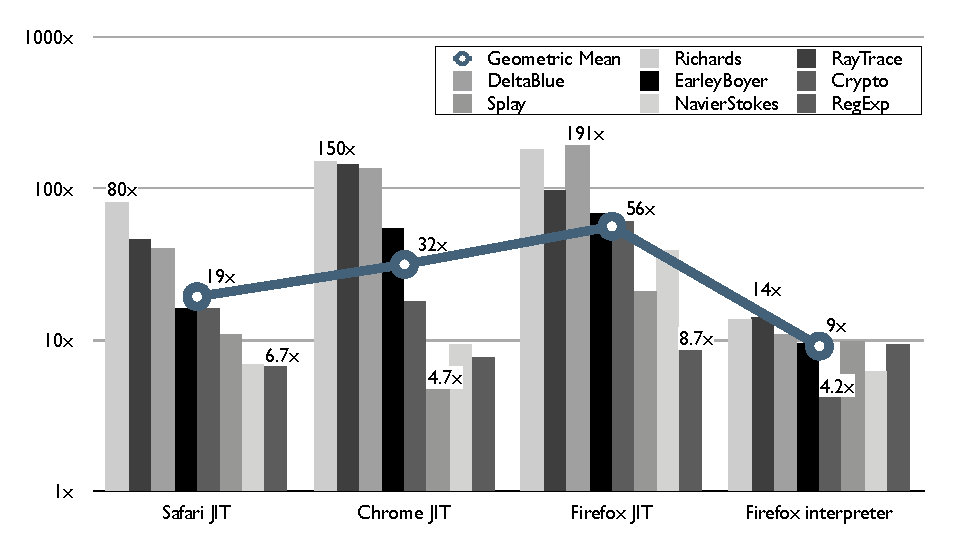
\includegraphics[width=.85\textwidth]{figures/InherentOverhead}
\caption[Inherent overhead of Photon]{Inherent overhead of Photon on the V8
benchmark suite on each JS VM. For each VM, the minimal and maximal slowdown
factors are shown near their corresponding benchmark.}
\label{fig:inherent-overhead-v8-benchmarks}
\end{center}
\end{figure}

Notably, the slowdown incurred on the Firefox interpreter is both lower, by a
factor of 2 to 6 times, and shows less variability, with a range of
$\approx$\factor{10} rather than $\approx$\factor{70} to $\approx$\factor{180},
than the slowdowns observed on other JIT-based VMs. We attribute these results
to the aggressive optimizations performed by JIT VMs, which are defeated by the
nature of the code transformation Photon performs. We performed another
experiment, whose results are not shown, where all function bodies were
enclosed in a \kw{try finally} statement, knowing that current compilers do not
optimize \kw{try} bodies. We then observed that the performance of the
JIT-based VMs became similar to that of the Firefox interpreter.

For JIT-based VMs, the important variablity of the results accross different
benchmarks illustrate partially the effect of the differential implementation
strategy for Photon (some operations of the language are reified while other
are simply directly reused). The effect is clear on the RegExp benchmark where
a significant part of the time is spent executing the matching algorithm of
regular expressions, which Photon directly reuse from the underlying VM.

For other benchmarks, the effect is less evident and the higher slowdowns can
be attributed to the ability of the JIT compiler to optimize the reified
operations.  Figure~\ref{fig:slowdown-vs-this-ratio} gives a rough
approximation of the nature of JavaScript operations performed by each
benchmark. Each pie slice area is proportional to the ratio of the number of
each of these operation performed during execution to the total number of
operations instrumented. For example, almost a quarter of all operations
counted for the Richards benchmark are accesses to the \kw{this} object, from
within a method. Although, NavierStokes and RegExp have a similar proportion of
object accesses (\kw{ObjectGetExpression}) compared to Richards, RayTrace and
DeltaBlue, a fifth compared to a fourth or a thirth, their execution time is
significantly faster, by at least an order of magnitude. It suggests some
operations such as array accesses are much better optimized than other object
accesses.

\begin{figure}[htbp]
\begin{center}
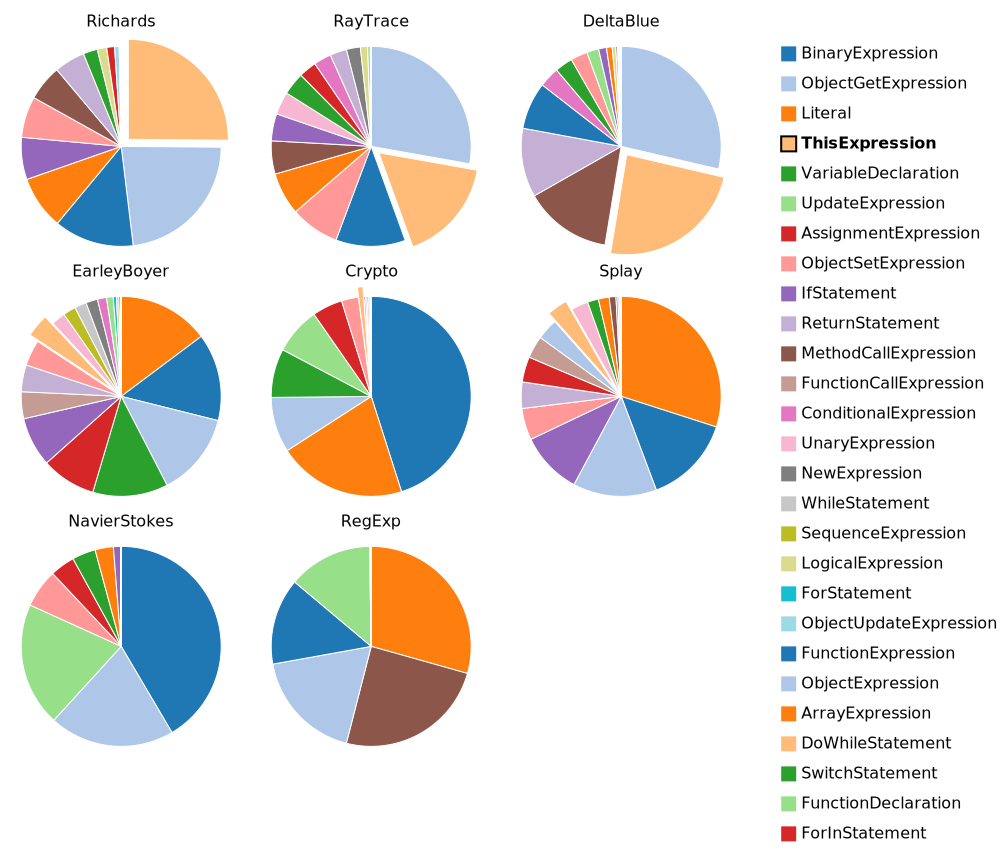
\includegraphics[width=.80\textwidth]{figures/benchmarkOperationRatios}
\caption[Ratios of operations for V8 benchmarks]{Comparison of the ratios of operations for the V8 benchmarks.}
\label{fig:operation-ratios}
\end{center}
\end{figure}

Comparing the frequency of each operations to the observed slowdown yielded a
confirmation of the validity of the differential strategy and an interesting
insight. For all control-flow operations, no clear correlation could be found,
which is unsurprising since the operations are not reified. However, of all the
operations observed, it is the frequency of the \kw{this} operation that seems
to correlate the most to the slowdowns observed.
Figure~\ref{fig:slowdown-vs-this-ratio} shows again the measured slowdowns,
grouped by benchmark and on a linear scale, and compares it to the ratio of
\kw{this} operations as in Figure~\ref{fig:operation-ratios}.  We attribute
thie correlation to the impact of the modification of the calling convention of
functions, in which the \kw{this} object is explicitly passed as an argument
instead of implicitly, as would be the case in the original JavaScript code. It
is likely that the compiler can optimize away type tests on operations using
the \kw{this} identifier within a method because it cannot be assigned,
therefore the object refered to remains constant throughout the method. This
can in turn facilitates, inlining of method calls using \kw{this} as the
receiver object.

\begin{figure}[htbp]
\begin{center}
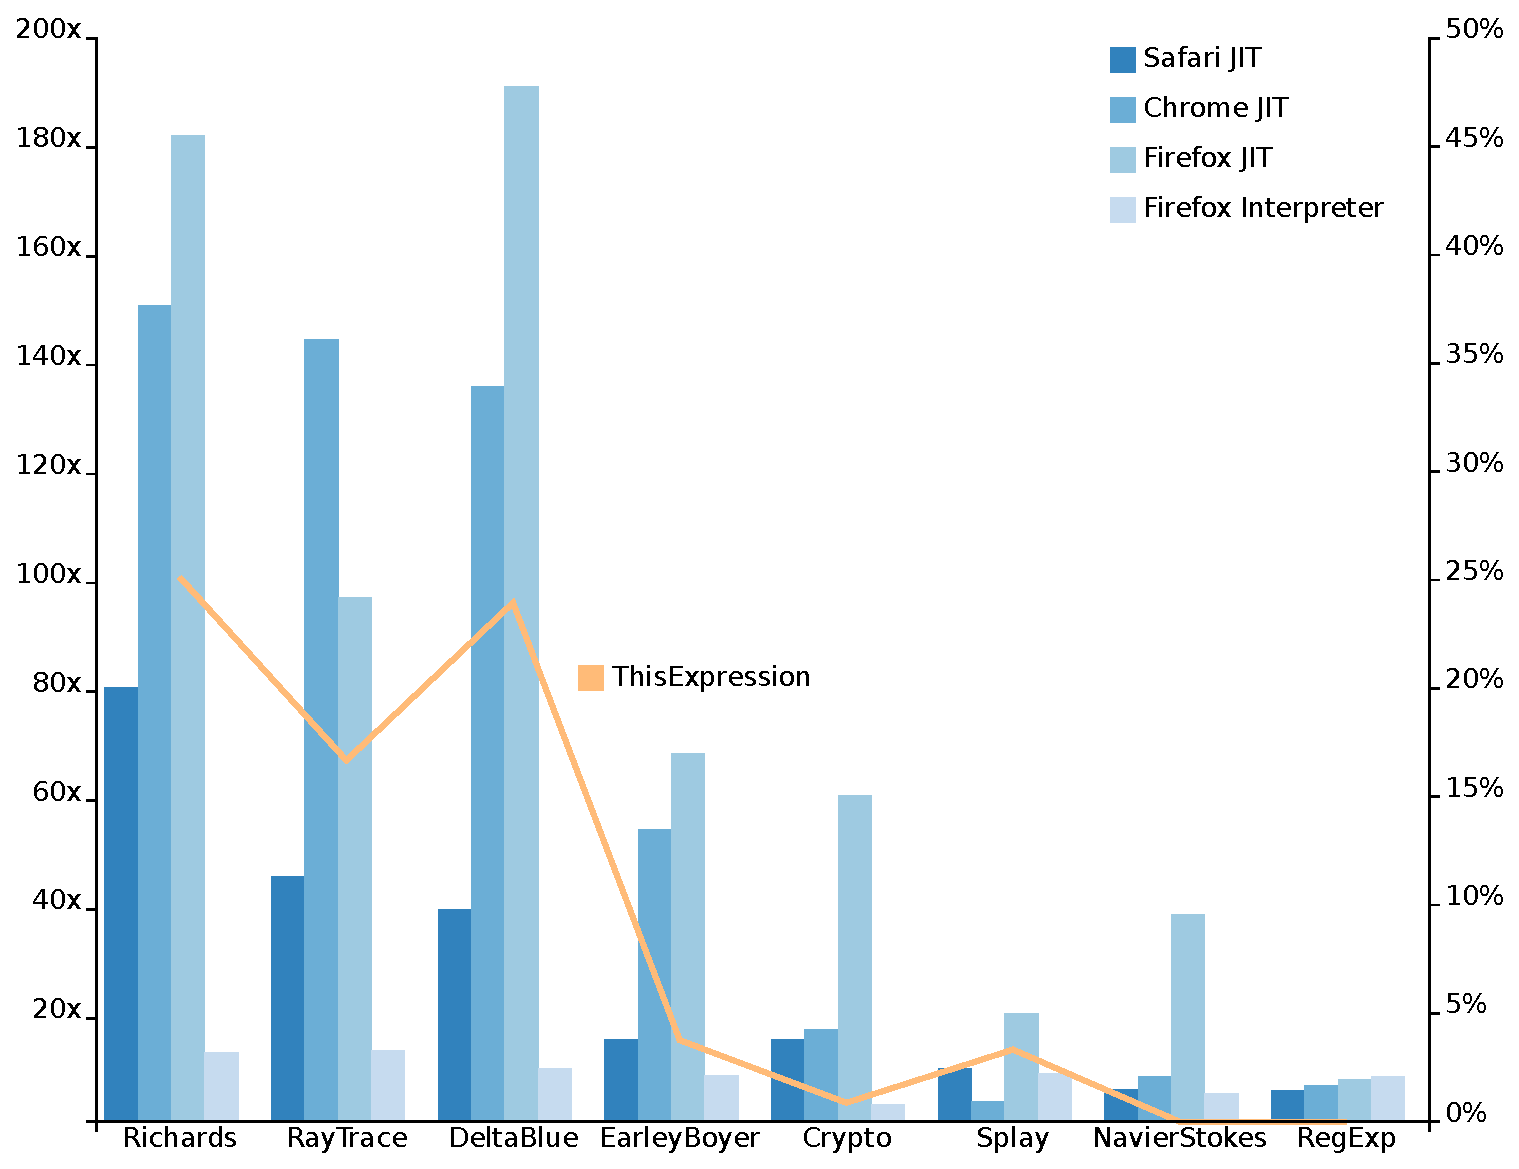
\includegraphics[width=.80\textwidth]{figures/slowdownVSThisRatio}
\caption[Slowdown vs Ratio of this operations]{Comparison of the inherent overhead of Photon with the measured ratio of \kw{this} operations during execution.}
\label{fig:slowdown-vs-this-ratio}
\end{center}
\end{figure}

\FloatBarrier

\section{Effect of send caching}

Figure~\ref{fig:send-cache-effect} illustrates the effect of the caching
strategy introduced in Section~\ref{sec:EfficientImplementation} by showing the
\textit{additional} slowdown incurred by disabling the optimization. These
figures should be \textit{multiplied} by the slowdowns shown in
Figure~\ref{fig:inherent-overhead-v8-benchmarks} to obtain the slowdowns
compared to the execution of the benchmarks without Photon. The EarleyBoyer
benchmark is not shown because its execution requires a stack size bigger than
the amount of stack space provided by the VMs.

\begin{figure}[htbp]
\begin{center}
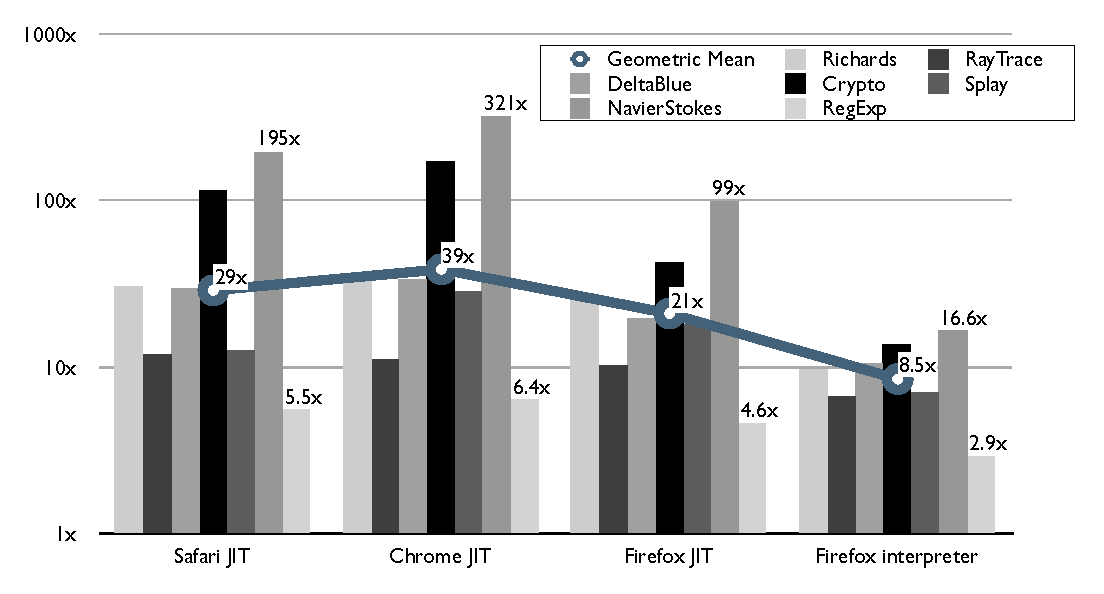
\includegraphics[width=.85\textwidth]{figures/effectSendCaches}
\caption[Execution speed slowdown of Photon with deactivated send caches]{Execution speed slowdown of Photon on the V8 benchmark suite on each JS VM when send caches are deactivated.}
\label{fig:send-cache-effect}
\end{center}
\end{figure}

Notice that the RegExp benchmark is the least affected, again because most of
the time is spent in the regular expression algorithms, unaffected by Photon's
transformation. The most affected benchmarks are NavierStokes and Crypto, both
performing a high number of array operations.

Needless to say, with a maximum additional slowdown of 320x and geometric means
between 8x and 40x, the caching optimization is critical to obtain acceptable
performance number.


\FloatBarrier

\section{Comparison with interpreter instrumentation}

The previous figures have shown the performance impact of Photon compared to a
bare execution on the same VM. However, a more interesting comparison is made
to the bare execution over an \textit{interpreter}, since Photon is intended to
replace instrumentation approaches that modify the implementation of a
state-of-the-art interpreter.

Figure~\ref{fig:perf-no-instrumentation-photon-vs-interpreter} shows the
relative speed of the benchmarks executing on Photon over the different
JIT-based VMs compared to the execution on the Firefox interpreter. A bar
smaller than one means that Photon is faster than the interpreter. Safari and
Chrome JITs perform almost equally well, with all but the RayTrace benchmark
being within a factor of two and an overall speed faster than the Firefox
interpreter. The Firefox JIT however is more than two times slower. Notice how
the NavierStokes and Crypto benchmarks are more than seven times \textit{faster}
than their interpreter counterpart, while performing object operations and
binary operations on numbers and strings. This is were the layered VM strategy
seems to really shines compared to the instrumentation of an interpreter, by
allowing the JIT to optimize through the additional abstraction layer.

The small performance difference between the Safari and Chrome JIT, but
significant in the worst case on the RayTrace benchmark, suggests prefering the
former if the browser implementation does not matter for a particular
instrumentation.



\begin{figure}[htbp]
\begin{center}
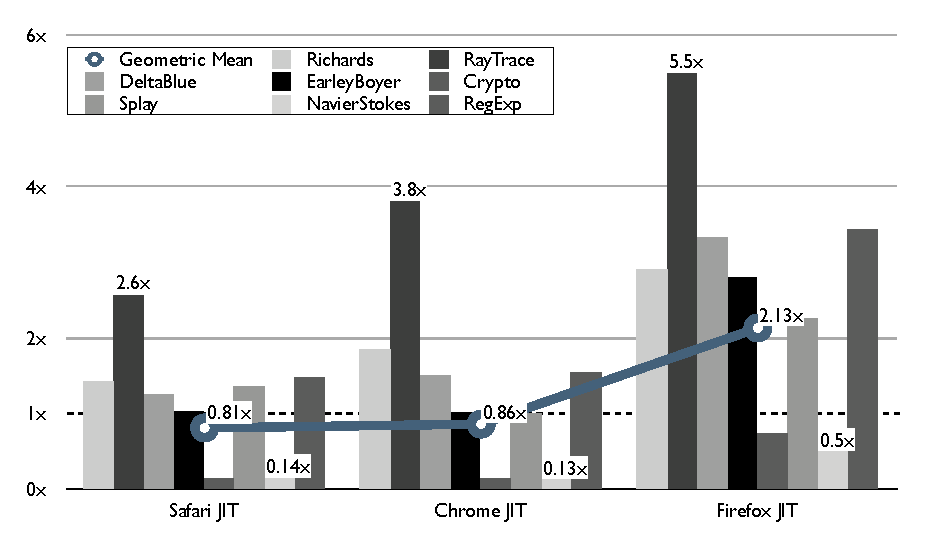
\includegraphics[width=.85\textwidth]{figures/ComparisonToInterpreter}
\caption[Performance of the V8 benchmark suite executed by Photon without instrumentation]{Performance of the V8 benchmark suite executed by Photon without instrumentation
on each JIT VM compared to the benchmark running directly on the Firefox interpreter.  The height of the bars
indicates the execution speed ratio (smaller than one is better for Photon).}
\label{fig:perf-no-instrumentation-photon-vs-interpreter}
\end{center}
\end{figure}

\FloatBarrier


\section{Performance with instrumentation}


Finally, we have evaluated the performance of Photon with an instrumentation
that counts the number of run-time occurrences of the following object
representation operations: property read, write and deletion. We chose this
particular instrumentation because it is simple, it covers frequently used
object model operations and it was actually used to gather information about JS
(it can be used to reproduce the object read, write and deletion proportion
figure from~\cite{behavior_js}).

Two implementations of this instrumentation were used; a simple and a
fast version.  The simple version does not exploit memoization and
corresponds to the straightforward implementation: incrementing a
counter and calling the corresponding object representation
operation. The fast version uses the memoization protocol to inline
the counter incrementations inside the optimized version of the object
operations.

The simple version is intended to measure the performance that can be
expected from a quickly developed instrumentation while the fast
version is intended to measure the performance impact of the
instrumentation operations alone. This is therefore a low-barrier
high-ceiling example and illustrates the flexibility that can be
gained when the choice of aiming for performance is left to users of
the system.  Not counting the result formatting code, the simple
version is 16 lines of JS code and the fast version is 100 lines of
JS code.

The execution speed slowdown of Photon on Safari is given in
Figure~\ref{fig:instr-slowdown}. The slowdowns for the simple version are
between \factor{1} and \factor{29} but are less than a factor of \factor{2} for
all the benchmarks with most benchmarks close to \factor{1}. This means that on
Safari JIT, on average, the benchmarks run with the fast version of the
instrumentation on Photon essentially at the same speed as the uninstrumented
original benchmarks directly on the Firefox interpreter.

\begin{figure}[htbp]
\begin{center}
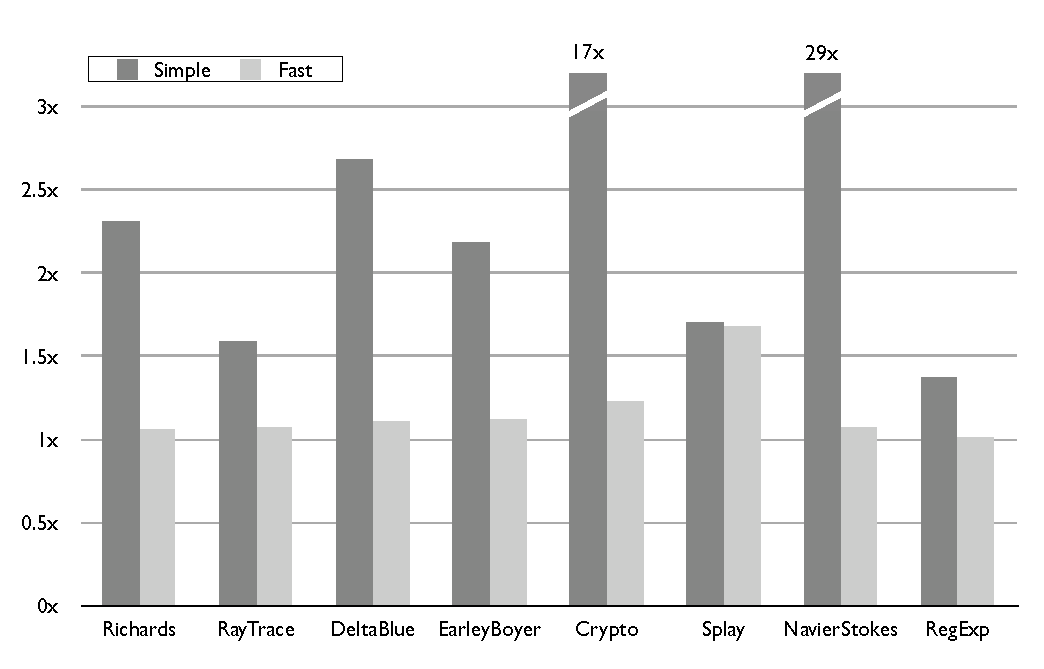
\includegraphics[width=.85\textwidth]{figures/InstrumentationSlowdown}
\caption[Execution speed slowdown of Photon with an instrumentation]{Execution
speed slowdown of Photon with a simple and a fast instrumentation of property
read, write and delete on the Safari VM.}
\label{fig:instr-slowdown}
\end{center}
\end{figure}


Results for other VMs are given  given in Tables~\ref{tb:slowdown-simple} and
\ref{tb:slowdown-fast}, showing that the results are similar for the Chrome
JIT. 


\FloatBarrier

%\section{Comparison to \textit{ad hoc} program transformation}
%\label{sec:esprof}
%
%As a final point of comparison, we have implemented an 
%\textit{ad hoc} source-to-source transformation that reifies the same
%operations as Photon, but in a more conventional way. The prototype
%implementation, esprof\footnote{\url{http://github.com/dufour/esprof}}
%allows instrumentations to register callbacks for various events. It does not
%allow for redefining the behavior of the reified operations, but exposes that
%same information to the callback as would be available in Photon. It is
%important to note that esprof has not been optimized for speed. It is meant to
%replicate the development effort required to implement a similar
%source-to-source transformation from a set of existing code manipulation tools, and
%emphasizes correctness of the transformation and ease of use over efficiency.
%
%\begin{figure}[htbp]
%\begin{center}
%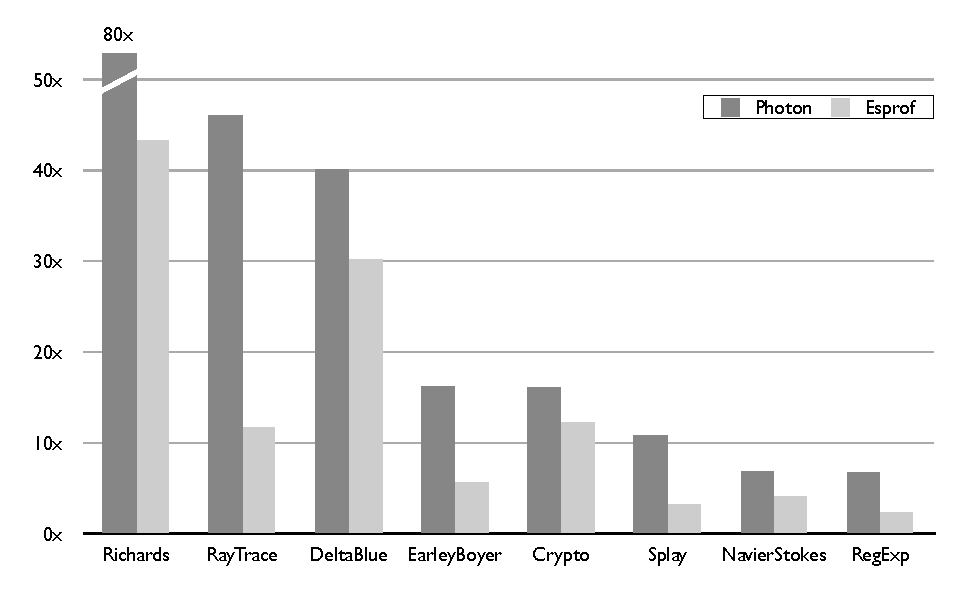
\includegraphics[width=.85\textwidth]{figures/PhotonVSEsprof}
%\caption[Execution speed slowdown of esprof vs photon]{Execution speed slowdown of the V8 benchmark suite transformed by esprof compared to photon.}
%\label{fig:esprof-slowdown}
%\end{center}
%\end{figure}
%
%Figure~\ref{fig:esprof-slowdown} shows the inherent overhead of esprof when
%executing the transformed program with no instrumentation being performed.
%esprof is on average a factor of \factor{2} faster than Photon on Safari JIT.
%However, this performance improvement comes at the cost of flexibility,
%expressiveness and, most importantly, isolation. Because esprof only reifies
%object operations performed on native JS objects, the burden of isolating the
%application from the effects of the instrumentation rests solely on the
%implementer of the instrumentation. Results for the other VMs are provided in
%Table~\ref{tb:esprof-slowdown}; esprof is faster on average by a factor between
%\factor{1.6} and \factor{3.3}.


%%% \subsection{Comparison to AspectScript}
%%% 
%%% ************ MOVE (A SUMMARY OF) THESE RESULTS TO THE RELATED WORK SECTION ********************
%%% 
%%% % (safari-photon / safari-aspectscript)
%%% \begin{table}[t]
%%% \centering
%%% \begin{tabular}{|l|rr|r|}
%%% \hline
%%%           & \multicolumn{2}{c|}{V8 Score}                             &       \\
%%%           & \multicolumn{1}{c}{without} & \multicolumn{1}{c|}{with}   &       \\
%%% Benchmark & \multicolumn{1}{c}{Photon}  & \multicolumn{1}{c|}{Photon} & Ratio \\
%%% \hline
%%% DeltaBlue    &     179 &       5 &\factor{  37.21} \\
%%% NavierStokes &    2265 &       5 &\factor{ 453.73} \\
%%% RegExp       &     568 &      56 &\factor{  10.06} \\
%%% Splay        &     973 &      35 &\factor{  27.73} \\
%%% \hline
%%% {\it Geom.~mean} & {\it  688} & {\it   15} & \factor{\it 46.59} \\ \hline
%%% \end{tabular}
%%% \caption{(safari-photon / safari-aspectscript)}
%%% %\label{tb:???}
%%% \end{table}
%%% % slowdown:  GEOMEAN = 135.20  MIN = 10.06  MAX = 1233.20


